\documentclass{article}
\usepackage[utf8]{inputenc}
\usepackage{enumerate}
\usepackage{graphicx}

\title{CS179N - Final Proposal}
\author{Christopher Yee\\ Rafael Gomez \\Lino Valdovinos  \\Kevin Lynn \\Jennifer Shin }
\date{April 20, 2018}


\begin{document}

\maketitle 


\begin{center}
{\huge Pixel Dawn}
\end{center}


\section{Story Line, Objective, and Tools}

An outbreak has occurred and 99\%\ of all living beings have turned into zombies. The player can choose from 4 different characters, each with their own back story (explained in section two). The objective of the game is to survive as long as possible, while killing as many zombies as possible. This game will be in 2D and will have aspects of run and gun, survival, and platforming. It will be a humorous, arcade-style game, and the story will be very minimal and not very impactful on the gameplay.
\\\\
The objective for the player is to survive as many waves of zombies as possible. In order to kill zombies the player will have weapons such as many different types of guns and throwable weapons like grenades. After each wave the amount of zombies that spawn will increase making each wave more difficult to pass.

We will use Unity as our game engine, and Gimp for creating our art.

\section{Character Back-stories}
There will be multiple characters that the player can choose from, each with their own unique abilities and back-story.

%\subsection{Ninja}
\begin{enumerate}

\item Ninja: Her father trained her with a katana, but then the zombies killed her father, so now she seeks revenge with father’s sword. 
%\subsection{Cyborg}

\item Cyborg: A failed military prototype for being too violent and was going to be destroyed, but escaped during the outbreak. He now kills the zombies for pleasure.
    
%\subsection{Little Girl}

\item Little Girl: A sadistic little girl who found her place in the apocalypse. She has a husky with a turret the follows here every where. 
    
%\subsection{Solider}

\item Soldier: He is a generic, patriotic soldier.
    
%\subsection{Zombies}

\item Zombies: These are the enemies. There are four types: Humans, bears, wolves, vultures.

\end{enumerate}

\section{Character Actions and Abilities}

All playable characters will be able to run and jump using WASD and Space. The player will use the mouse to aim their weapons and attack. However, each character will have their own special abilities, both passive and activatable.

\begin{enumerate}
    
%\subsection{Ninja}

\item Ninja: She will be able to double jump and jump off walls. This character will be the most mobile of the four classes, but has little to few offensive abilities, including dashes and sword strikes.

%\subsection{Cyborg}

\item Cyborg: He will be able to fly for short periods of time. This character will deal more damage while in the air, due to having activatable abilities only available while airborne.
    
%\subsection{Little Girl}

\item Little Girl: She moves slow, but her dog that follows her around can equip a weapon as well. She has spikes in power when she has a tantrum. Her activatable abilities will involve her dog and her screams.
    
%\subsection{Solider}

\item Soldier: He is able to run quickly on the ground and attacks with his weapons at a faster rate. He is the most "basic" of the characters, having very similar mechanics to soldier characters in other games. His activatable abilities include air strikes and explosives.

\end{enumerate}

\begin{center}
    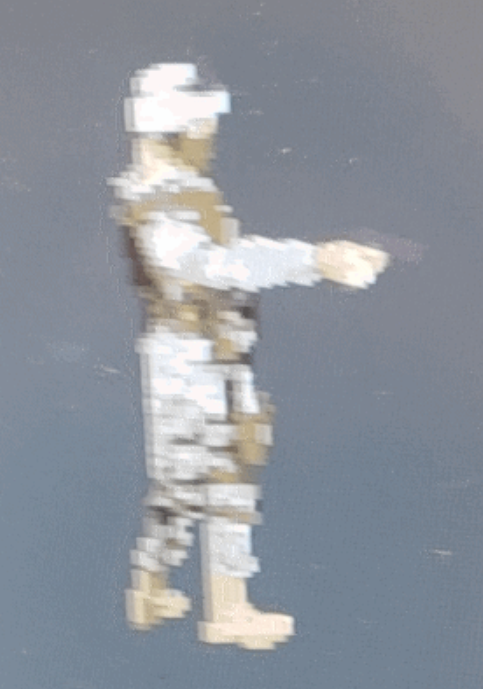
\includegraphics[width = 2in]{solider.PNG}\\
    Figure 1: Soldier Sprite
\end{center}
    
\section{Art}
    The game will be made in pixel art, some of the assets will be obtained from free to uses assets online, and other more specific assets will need to be made.  The art for the character will required to have a separate sprite from the body and the arms so the that arms can hold weapons and aim all around them. The art for the world will be determined by the assets that are available to us. 


\section{Character Interactions}
Characters have lives that will decrease when hit, and the game is over when you have 0 lives. The game is only single player.


\section{World Interactions}

    Every playable character can interact with a vendor NPC to purchase weapons from, power ups, and health. The store uses in game currency obtained from killing zombies. There are also be stairs and ladders that the playable character can use traverse the level.

\section{Character AI}


\begin{enumerate}
  \item Zombie Humans: are slow moving and only have melee attack but come in growing mobs. 
  \item Zombie Wolves: are fast moving, aggressive, but are easy to kill.
  \item Zombie Bats: are able to fly and attack from any direction.
  \item Zombie Bear: has a lot of health and therefore it is difficult to kill. In addition, he does alot of damage, "Boss Enemy" 
\end{enumerate}

\section{Priorities}
Scale (1-5) were (1) is high priority and (5) is low priority. 
\begin{enumerate}[(i)]
    \item World interactions: Complete map art and design (1), Basic Combat and Damage Mechanic (1), Character Movement Mechanics(1), In game store using in-game currency (2), Guns(2), Character Sounds(3), Gun sounds(2), Enemy sounds(2), In game item iterations e.g. Player health packets (3), Enemy Spawns (1), Ladders or Springs(3), Activate Abilities (3).
    \item Enemy type Models and Animations: Human zombie (1), Zombie Wolves (2), Zombie Bats (3), Zombie Bear (4),
    \item Character Models and Animations: Solider (1), Little girl (2), Ninja (3), Cyborg (4),
    \item Other: Game Menu(1), Game Menu Music (3), High score tracker (5), Player life bar (1),
\end{enumerate}


\section{Milestones}
\subsection{Milestone 1}
    Basic movements around, one character model sprite with basic animation, like running, jumping, shooting, and collision with the ground and walls.
    In addition, basic sprite models for ground and background will be made.
\smallskip

\textbf{List of Interactions and Tasks:}

\begin{enumerate}
     \item Main Menu
        \begin{enumerate}
            \item Menu Options: Start and Exit
            \item Menu Music
            \item Character Selection Screen
            \item Stage Selection Screen
            \item High Score
        \end{enumerate}
    \item Characters
        \begin{enumerate}
            \item Movement with WASD and Space
            \item Gun arm moves with mouse, and left click fire the weapon
            \item Ninja - Sprite, Double Jump, Jump off walls
            \item Cyborg - Sprite, Flying by holding space
            \item Little Girl - Sprite, Dog, Tantrum Power-up
            \item Soldier - Sprite, Faster running and Faster attack rate
            \item Sounds - Character occasional pain sounds when injured, beginning of level dialogue
            \item Personalized offensive abilities for each character, like air strikes for the Soldier (low priority).
        \end{enumerate}
    \item Enemies
        \begin{enumerate}
            \item Human - Sprite, Walking animation, Walks towards player
            \item Wolves - Sprite, Faster walk speed, Less health
            \item Bats - Sprite, Flies erratically, Little health
            \item Bear - Sprite, Slower walking, More health
            \item Sounds - Groans, Yells
            \item Enemies randomly spawn from the edges of the map or somewhere in the level where the player isn't
        \end{enumerate}
    \item World and Other
        \begin{enumerate}
            \item Base Mansion Level
            \item Useable Ladders
            \item Level Music
            \item In-game currency gained by killing zombies
            \item Vendor where the player can spend currency to buy new weapons
            \item Guns: Pistol, Machine Gun, Explosives
            \item Gun Sounds
            \item Character UI (Inventory, lives, money)
            \item Increasing enemy difficulty as time goes on (more spawns, different types of enemies start to appear)
            \item Power Ups
            \item Health Packs
            \item Game Over Screen
        \end{enumerate}
\end{enumerate}
    
    We will take a small video of our character interacting with a simple world model, like him walking around, to document our progress and upload it to ilearn. 
\subsection{Milestone 2}
    Gun interactions and mouse aiming. Make an enemy to shoot at, and have the enemy move towards the player. More level details and more characters. Menu for selecting characters. 
    \\We will take a small video of our character moving and shooting with one gun model at zombie enemy to document our progress and upload it to ilearn. 
\subsection{Milestone 3}
    Fully functional level, not including enemy spawns. All sprites will be made by now. Main Menu done as well.
    \\We will take a  video of our showcasing the main menu as well as the character traversing the whole level. If the different characters aren't able to be selected from the menu yet, then we will send separate pictures of the other sprites.

\subsection{Milestone 4}
    Character specific abilities finished, basic zombie AI for all types. And game sounds including intro music, in-game music, gun sounds, enemy sounds, and other game-play sounds.  
    \\We will take a video showcasing the characters special abilities  video of our character interacting with one gun model and an enemy with sound to document our progress and upload it to ilearn. 

\subsection{Milestone 5}
    All weapons available, and game shop fully functional using in-game currency obtain from kills to purchase weapons and health.
    \\We will take a video showcasing the complete game to document our completion and upload it to ilearn. 
\end{document}
